\chapter{Analyse}

\section{Introduction}

Dans ce chapitre, on va résoudre 3 problèmes en utilisant les approches classiques d'apprentissages profonds, et aussi avec les réseaux de neurones binarisés.
On va essentiellement résoudre:
\begin{enumerate}
	\item Régression de $f:x\rightarrow 2x^2+3x+2$ sur $[-4,4]$
	\item Classification des chiffres en exploitant le jeu de données MNIST
	\item Classification des chiffres en exploitant le jeu de données Free Spoken Digits
\end{enumerate} 
\newpage
\section{Méthodologie adoptée}
Dans les problèmes, qui se suivent, nous avons suivi la méthodologie CRSIP-DM\cite{11}.
\subsection{CRISP-DM}
CRISP-DM signifie Cross Industry Standard Process for Data Mining (CRISP-DM) est une méthode mise à l'épreuve sur le terrain permettant d'orienter les travaux d'exploration de données. 
\subsubsection{Cycle CRISP-DM}

\begin{enumerate}
	\item Connaissance du métier.
	\item Connaissance des données.
	\item Préparation des données.
	\item Modélisation des données.
	\item Évaluation.
	\item Déploiement.
\end{enumerate}
\begin{figure}[h!]
	\centering
	\includegraphics[width=.5\textwidth]{Figures/CRISP-DM.png}
	\caption{Méthodologie CRISP-DM}
	\label{fig:CRSIP-DM}
\end{figure}
\FloatBarrier
\newpage
\section{Régression de $f:x\rightarrow 2x^2+3x+2$ sur $[-4,4]$}
\subsection{Importance}
Ce problème est fait artificiellement étudier la robustesse les  BNNs implémentées.
\subsection{Jeux de données}
Dans cette problématique, le jeu de données est généré avec $n=20000$ exemplaires:
\begin{itemize}
	\item $x_1,\dots,x_n \sim \mathcal{U}(-4,4)$ 
	\item $\epsilon_1,\dots,\epsilon_n \sim \mathcal{N}(0,0.1)$
	\item $y_1,\dots,y_n$ avec $y_i=f(x_i)+\epsilon_i\quad \forall i\in\{1,\dots,n\}.$ 
\end{itemize}

\subsection{Modèle}
Notre modèle $\mathcal{M}_\theta$ est un estimateur de $f$ paramétrisé par $\theta\in S$. L'ensemble $S$ va dépendre de type du modèle.
\newline
Dans notre cas, l'architecture du modèle est décrite par la figure ci-dessous.

Pour la binarisation, nous avons utilisé la fonction $\sign$ dans la propagation avant, et nous avons utilisé la méthode STE bornée sur $[-1,1]$ pour la propagation en arrière.

\subsection{Hypothèses}
On a fait les hypothèses suivantes:
\begin{enumerate}
	\item H1: $x_1,\dots,x_n$ sont mutuellement indépendents
	\item H2: Les bruits sont mutuellement indépendentes.
	\item H3: Le model $\mathcal{M}$ ne connaît sur la fonction $f$ que $f(x_i)\approx y_i,$et il ne tient pas compte de l'erreur $\epsilon_i.$
\end{enumerate}
\subsection{Problème Formel}
On va chercher $\theta^*$ tel que:
\begin{equation}\label{Regression:MSE}
	\theta^* = \argmin_{\theta \in S } \lVert\boldsymbol{y}-\mathcal{M}_\theta(\boldsymbol{x})\rVert_2^2 =\argmin_{\theta \in S }\sum_{i=1}^n(y_i-\mathcal{M}_\theta(x_i))^2
\end{equation}

\subsection{Entraînement}
On a entraîné 3 types de modèles:
\begin{itemize}
	\item BinaryNet
	\item XnorNet
	\item ABCNet
\end{itemize}
Pour chacun, on a utilisé:
\begin{itemize}
	\item L'optimiseur Adam, avec $\mathtt{learning\_rate}=10^{-2}$ et $\mathtt{decay}=10^{-4}$
	\item La fonction objective MSE comme décri dans l'équation \eqref{Regression:MSE}
	\item Taille de lot égale à $128$
	\item Une limite de $30$ époches.
	.
\end{itemize}
\subsection{Performances de prédiction}
On a tracé la courbe de chaque modèle en le comparant avec $f$:
\begin{figure}[h!]
	\centering
	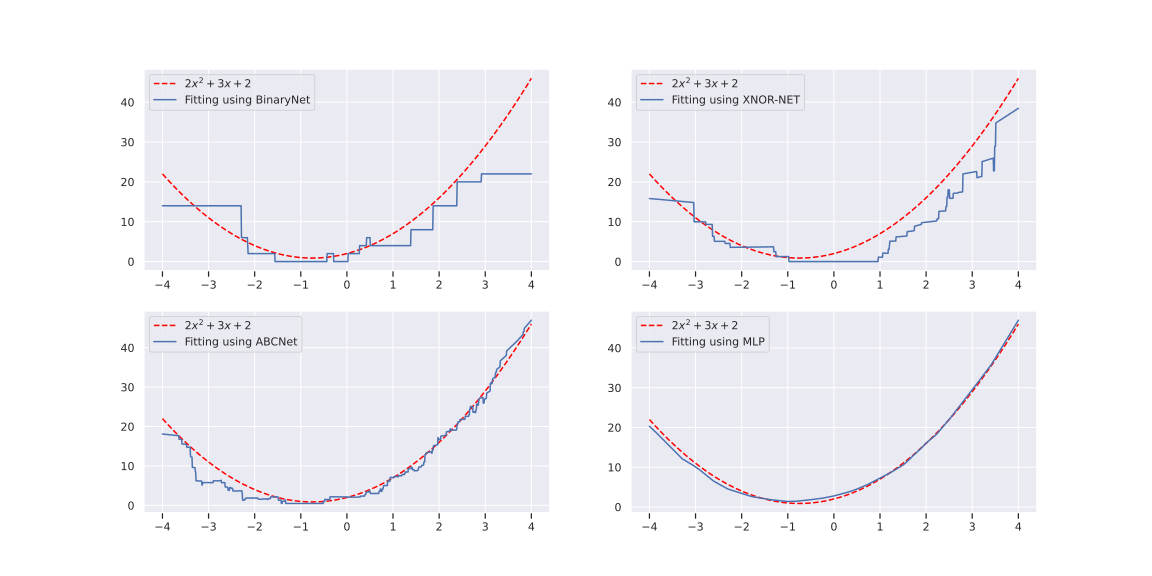
\includegraphics[width=1\textwidth]{Figures/RegressionPerformance.png}
	\caption{Courbe de chaque modèle}
	\label{fig:Regression-Curve}
\end{figure}
\FloatBarrier
Pour mesurer la qualité de régression, nous avons utilisé 3 métriques:
\subsubsection{Distance $\mathscr{L}^\infty$}
C'est la distance $\mathscr{L}^\infty$ dans l'espace des fonctions continues $\mathscr{C}([-4,4])$:
\begin{equation}
	\mathscr{L}^\infty_{\text{test}}(y,\mathcal{M}_\theta)=\sup_{x\in[-4,4]}\lvert \mathcal{M}_\theta(x)-f(x) \rvert
\end{equation}
\subsubsection{Distance $\mathscr{L}^1$}
C'est la distance $\mathscr{L}^1$ dans l'espace $\mathscr{C}([-4,4])$:
\begin{equation}
	\mathscr{L}^1_{\text{test}}(y,\mathcal{M}_\theta)=\int_{-4}^4 \lvert\mathcal{M}_\theta(x)-f(x)\rvert dx
\end{equation}
\subsubsection{Distance $\mathscr{L}^2$}
C'est la distance $\mathscr{L}^2$ dans l'espace $\mathscr{C}([-4,4])$:
\begin{equation}
	\mathscr{L}^2_{\text{test}}(y,\mathcal{M}_\theta)=\left(\int_{-4}^4 \left(\mathcal{M}_\theta(x)-f(x\right))^2 dx\right)^{\frac{1}{2}}
\end{equation}
Dans la pratique, nous allons estimer les 2 intégrales en utilisant la méthode Romb avec $n=2^{20}+1$ points.
\newline 
On a trouvé les résultats suivant:
\newline

\begin{tabularx}{\textwidth}{| X | X | X | X | X |}
	\hline
	
	Modèle & $\mathscr{L}^\infty$ & $\mathscr{L}^1$ & $\mathscr{L}^2$ Carré & $\mathscr{L}^2$  \\
	\hline
	BinaryNet & 24.000 & 4.322 & 42.524 & 6.521 \\
	\hline 
	XNOR-NET & 13.852 & 3.531 & 19.671 & 4.435 \\
	\hline
	ABCNet & 7.395 & 1.421 & 4.024 & 2.01 \\
	\hline
	MLP & 1.692 & 0.616 & 0.562 & 0.750 \\
	\hline
\end{tabularx}
Dans le tableau ci-dessus, MLP est le modèle classique sans utilisation de binarisations, et il sert comme reférence.

\FloatBarrier
\newpage
\section{Classification MNIST}
\subsection{Introduction}
MNIST\cite{12} est un jeu de données des images de chiffres écrits à la main. Il admet:
\begin{itemize}
	\item $60000$ exemplaires pour l'entraînement
	\item $10000$ exemplaires pour le test.  
\end{itemize}
Les images sonts de tailles $28\times 28$ et en niveau de gris, dans lesquels les chiffres sont centrés.

Ce jeu de données sert comme un test de performance des modèles de Machine Learning.

\begin{figure}[h!]
	\centering
	\includegraphics[width=.4\textwidth]{Figures/mnist-3.0.1.png}
	\caption{Des images de MNIST}
	\label{fig:MNIST-Sample}
\end{figure}

\subsection{Topologie}
Nous avons utilisé l'architecture ci-dessous:
\begin{figure}[h!]
	\centering
	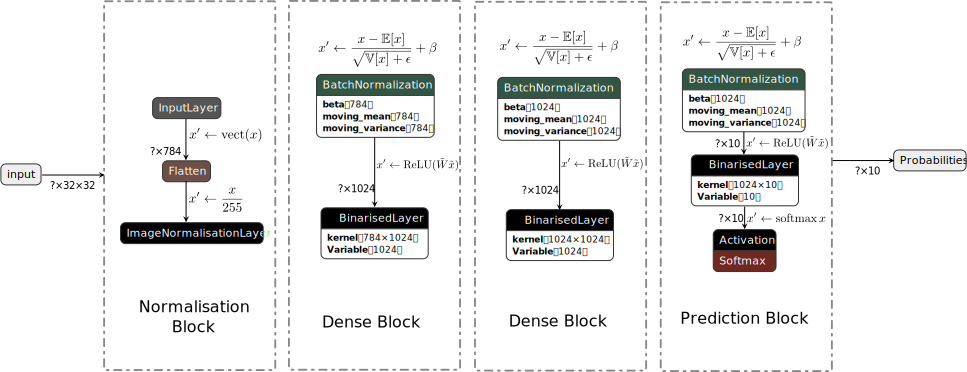
\includegraphics[width=1\textwidth]{Figures/MNIST-Topology.png}
	\caption{Architecture du modèle MNIST}
	\label{fig:MNIST-Topology}
\end{figure}
\FloatBarrier
BinarisedLayer désigne ici le type de couche dense binariséé qui est utilisé. Il s'agit de:
\begin{itemize}
	\item QuantDense pour BinaryNet
	\item ScaledQuantDense pour XnorNet
	\item ABCDense pour ABCNet
\end{itemize}
Dans la figure, les dimensions de couche sont décrits explicitement avec leurs équations, et le point d'interrogation '?' indique que le modèle est indifférent à la taille de lot.
\subsection{Modèle}
On avons utilisé $3$ modèles pour l'architecture donnée:
\begin{itemize}
	\item BinaryNet, avec:
	\subitem Binarisation: $\sign$ avec STE
	\subitem Activation: ReLU
	\item XnorNet, avec:
	\subitem Binarisation: $\sign$ avec STE
	\subitem Activation: ReLU
	\subitem $\alpha$ et $\beta$ sont calculés par produit scalaire.
	\subitem Le facteur $\alpha$ est entraînable, initialisé à \eqref{XnorNet:InnerProductQuantification:Result}
	\subitem Le facteur $\beta$ est calculé, initialisé à \eqref{XnorNet:InnerProductQuantification:Result}
	\item ABCNet avec:
	\subitem Binarisation: $\sign$ décalée avec STE.
	\subitem Activation: ReLU.
	\subitem $n=3$ binarisations des poids, suivant 
	\subitem $m=1$ binarisations des noeuds, suivant
	\subitem $\mu_i$ et $\kappa_j$ sont entraînables
	\subitem $\alpha_i$ et $\beta_j$ sont calculés par produit scalaire.
	
\end{itemize}
\subsection{Performances de prédictions}
\subsection{Performance mémoire}
les performances mémoire sont mésurées avec la taille totale des paramètres, qui donnent une approximation de l'utilisation mémoire du modèle à son déploiement.
\newline Nous avons fait la comparaison de $2$ versions de chaque modèle:
\begin{itemize}
	\item Les paramètres (non-binarisés) sont en float à 32 bits.
	\item Les paramètres (non-binarisés) sont en float à 8 bits.
\end{itemize}
\subsubsection{Comparaison Float 32}
Les paramètres de type float sont naturellement encodés en $64 \ \text{bits}$ dans TensorFlow. En apportant des binarisations, on va avoir le tableau suivant
\begin{table}[h]
	\begin{tabularx}{\textwidth}{| X | X | X | X | X |}
		\hline
		
		Modèle & Nombre de paramètres binarisés &  Nombre de paramètres non-binarisés &  Taille de mémoire en \text{KB} \newline $T$ &  Taux de compression $\tau=\frac{T_{\text{MLP}}}{T_{\text{Model}}}$ \\
		\hline
		MLP & 0 & 1'869'354 & 7302.16 & 1 \\
		\hline 
		BinaryNet & 1'861'632 & 5'664 & 249.38 & 29.28 \\
		\hline
		XnorNet & 1'861'632 & 7'722 & 257.41 & 28.36 \\
		\hline
		ABCNet & 5'584'896 & 11'838 & 727.99 & 10.03 \\
		\hline
	\end{tabularx}
	\caption{Comparaison entre les modèles en utilisant Float32 }
\end{table}
\FloatBarrier
\subsubsection{Comparaison Float 8}
On peut aussi compresser les paramètres float en utilisant Float 8 (Minifloat) dans TensorFlow.
\newline Ainsi, on va avoir le tableau suivant:
\begin{table}[h]
	\begin{tabularx}{\textwidth}{| X | X | X | X | X |}
		\hline
		
		Modèle & Nombre de paramètres binarisés &  Nombre de paramètres non-binarisés &  Taille de mémoire en \text{KB} \newline $T$ &  Taux de compression $\tau=\frac{T_{\text{MLP}}}{T_{\text{Model}}}$ \\
		\hline
		MLP & 0 & 1'869'354 & 7302.16 & 1 \\
		\hline 
		BinaryNet & 1'861'632 & 5'664 & 249.38 & 29.28 \\
		\hline
		XnorNet & 1'861'632 & 7'722 & 257.41 & 28.36 \\
		\hline
		ABCNet & 5'584'896 & 11'838 & 727.99 & 10.03 \\
		\hline
	\end{tabularx}
	\caption{Comparaison entre les modèles en utilisant Float8 }
\end{table}
\FloatBarrier

\subsubsection{Quantification de Float 32 à Float 8}
Avec les deux tableaux précédents, on peut étudier l'apport de la réduction de précision de float à minifloat pour les $4$ modèles considérés en terme de mémoire.
\begin{table}[h]
	\begin{tabularx}{\textwidth}{| X | X | X | X |}
		\hline
		
		Modèle & Taille avec Float 32\newline $T_{32}$ &  Taille avec Float 8  \newline $T_8$&  Rapport de Taille \newline $\tau=\frac{T_{\text{8}}}{T_{\text{32}}}$ \\
		\hline
		MLP & 7302.16 & 1825.54 & 0.25 \\
		\hline 
		BinaryNet & 249.38 & 232.78  & 0.9334 \\
		\hline
		XnorNet & 257.41 & 234.79 & 0.9121 \\
		\hline
		ABCNet & 727.99  & 693.31 & 0.9523\\
		\hline
	\end{tabularx}
	\caption{Comparaison entre les modèles en utilisant Float8 }
\end{table}
\FloatBarrier

\subsection{Performance temps}
les performance temps sonts mésurée avec le nombre d'instructions multiply \& accumulate (MAC) nécessaires pour chaque modèle à son déploiement.


\begin{tabularx}{\textwidth}{| X | X | X | X | X | X |}
	\hline
	
	Modèle & Nombre de MACs binarisés\newline $N_B$ &  Nombre de MACs non-binarisés \newline $$N_F$$ &  Instructions équivalentes: \newline $$I=\frac{N_B}{64}+N_F$$ &  Taux de MACs binarisés \newline $$\alpha=\frac{N_B}{N_B+N_F}$$ & Taux de gain: \newline $$\tau=\frac{I_{\text{MLP}}}{I_{\text{Model}}}$$ \\
	\hline
	MLP & 0 & 1’861’632 & 1’861’632 & 0 & 1 \\
	\hline 
	BinaryNet & 1'861'632 & 2058 & 29'088 & 1 & 64 \\
	\hline
	XnorNet & 1'861'632 & 7'722 & 31'064 & 0.9989 & 59.92 \\
	\hline
	ABCNet & 5'584'896 & 11'838 & 93'438 & 0.9989 & 19.92 \\
	\hline
\end{tabularx}


\newpage
\section{Classification Free Spoken Digits}
\subsection{Importance}
Dans la littérature, les BNNs utilisés principalement avec les jeux de données images. Ainsi, notre objectif est l'utilisation d'un BNN pour résoudre les problèmes de traitement des signaux à faible complexité.
\newline Nous avons choisis Free Spoken Digits\cite{13} comme une preuve de concept de l'applicabilité des BNNs dans ce genre de problèmes. De plus, nous allons utiliser l'expertise de dB Sense pour extraire intelligemment les informations utiles d'une parole afin de construire un classificateur performant et à faible complexité. 
\subsection{Introduction}
Free Spoken Digits\cite{13} (FSD) est un jeu de données audio qui consiste d'un ensemble de fichiers wav à une fréquence d'échantillonage de $8 \ \text{kHz}$. Les fichiers sont coupés pour minimiser le silence.
\begin{figure}[h!]
	\centering
	\includegraphics[width=.7\textwidth]{Figures/free-spoken-digits-4.png}
	\caption{Des images de MNIST}
	\label{fig:FreeSpokenDigits-Sample}
\end{figure}
\newpage
\subsection{Structure}
FSD est enrigistré à l'aide d'un microphone monophonique, et il admet $6$ orateurs qui ont chacun $50$ enregistrements par chiffre.
\newline En total, chaque orateur admet $500$ enregistrements, et donc ce jeux de données admet $3000$ fichiers audio.
\newline De plus, chaque enregistrement admet un nom significatif de la forme \texttt{digit\_person\_id.wav} avec:
\begin{itemize}
	\item \texttt{digit} est le chiffre prononcé dans l'enregistrement.
	\item \texttt{person} est le nom de l'orateur.
	\item \texttt{id} est l'identificateur de l'enregistrement, sachant la personne et le chiffre, appartenant à l'ensemble $\{0,\dots,49\}$
\end{itemize}
\subsection{Analyse}
